\section{Background}
\label{sec:background}

\subsection{Single-Input Multiple-Output}
\label{sec:simo}

Wireless devices have transitioned to using multiple antennas to leverage gains from on both client devices and access points.
These are known as multiple-input multiple-output (MIMO) systems and their design involves using simultaneous transmissions and receptions from different antennas to obtain higher throughput, than what would be possible using any given pair of antennas on a transmitter and receiver.
MIMO systems can provide higher throughput and resilience due to their ability to coherently combine signals both at the transmitter (known as \textit{beamforming}) and the receiver (known as \textit{diversity}).
In traditional MIMO system such as those found in 802.11n, the various receiver antennas are a part of the same device which makes it easier to synchronize and combine the different receiver channels.
However, distributed MIMO systems allow the receivers to be completely independent devices and still be able to coherently combine the received signals.
Single-input multiple-output (SIMO) as shown in \figref{simo} is a subset of distributed MIMO systems where the transmitter only uses a single antenna.
The LoRaWAN scenario we explore in this paper is based on SIMO systems.

\begin{figure}[!htb]
    \centering
    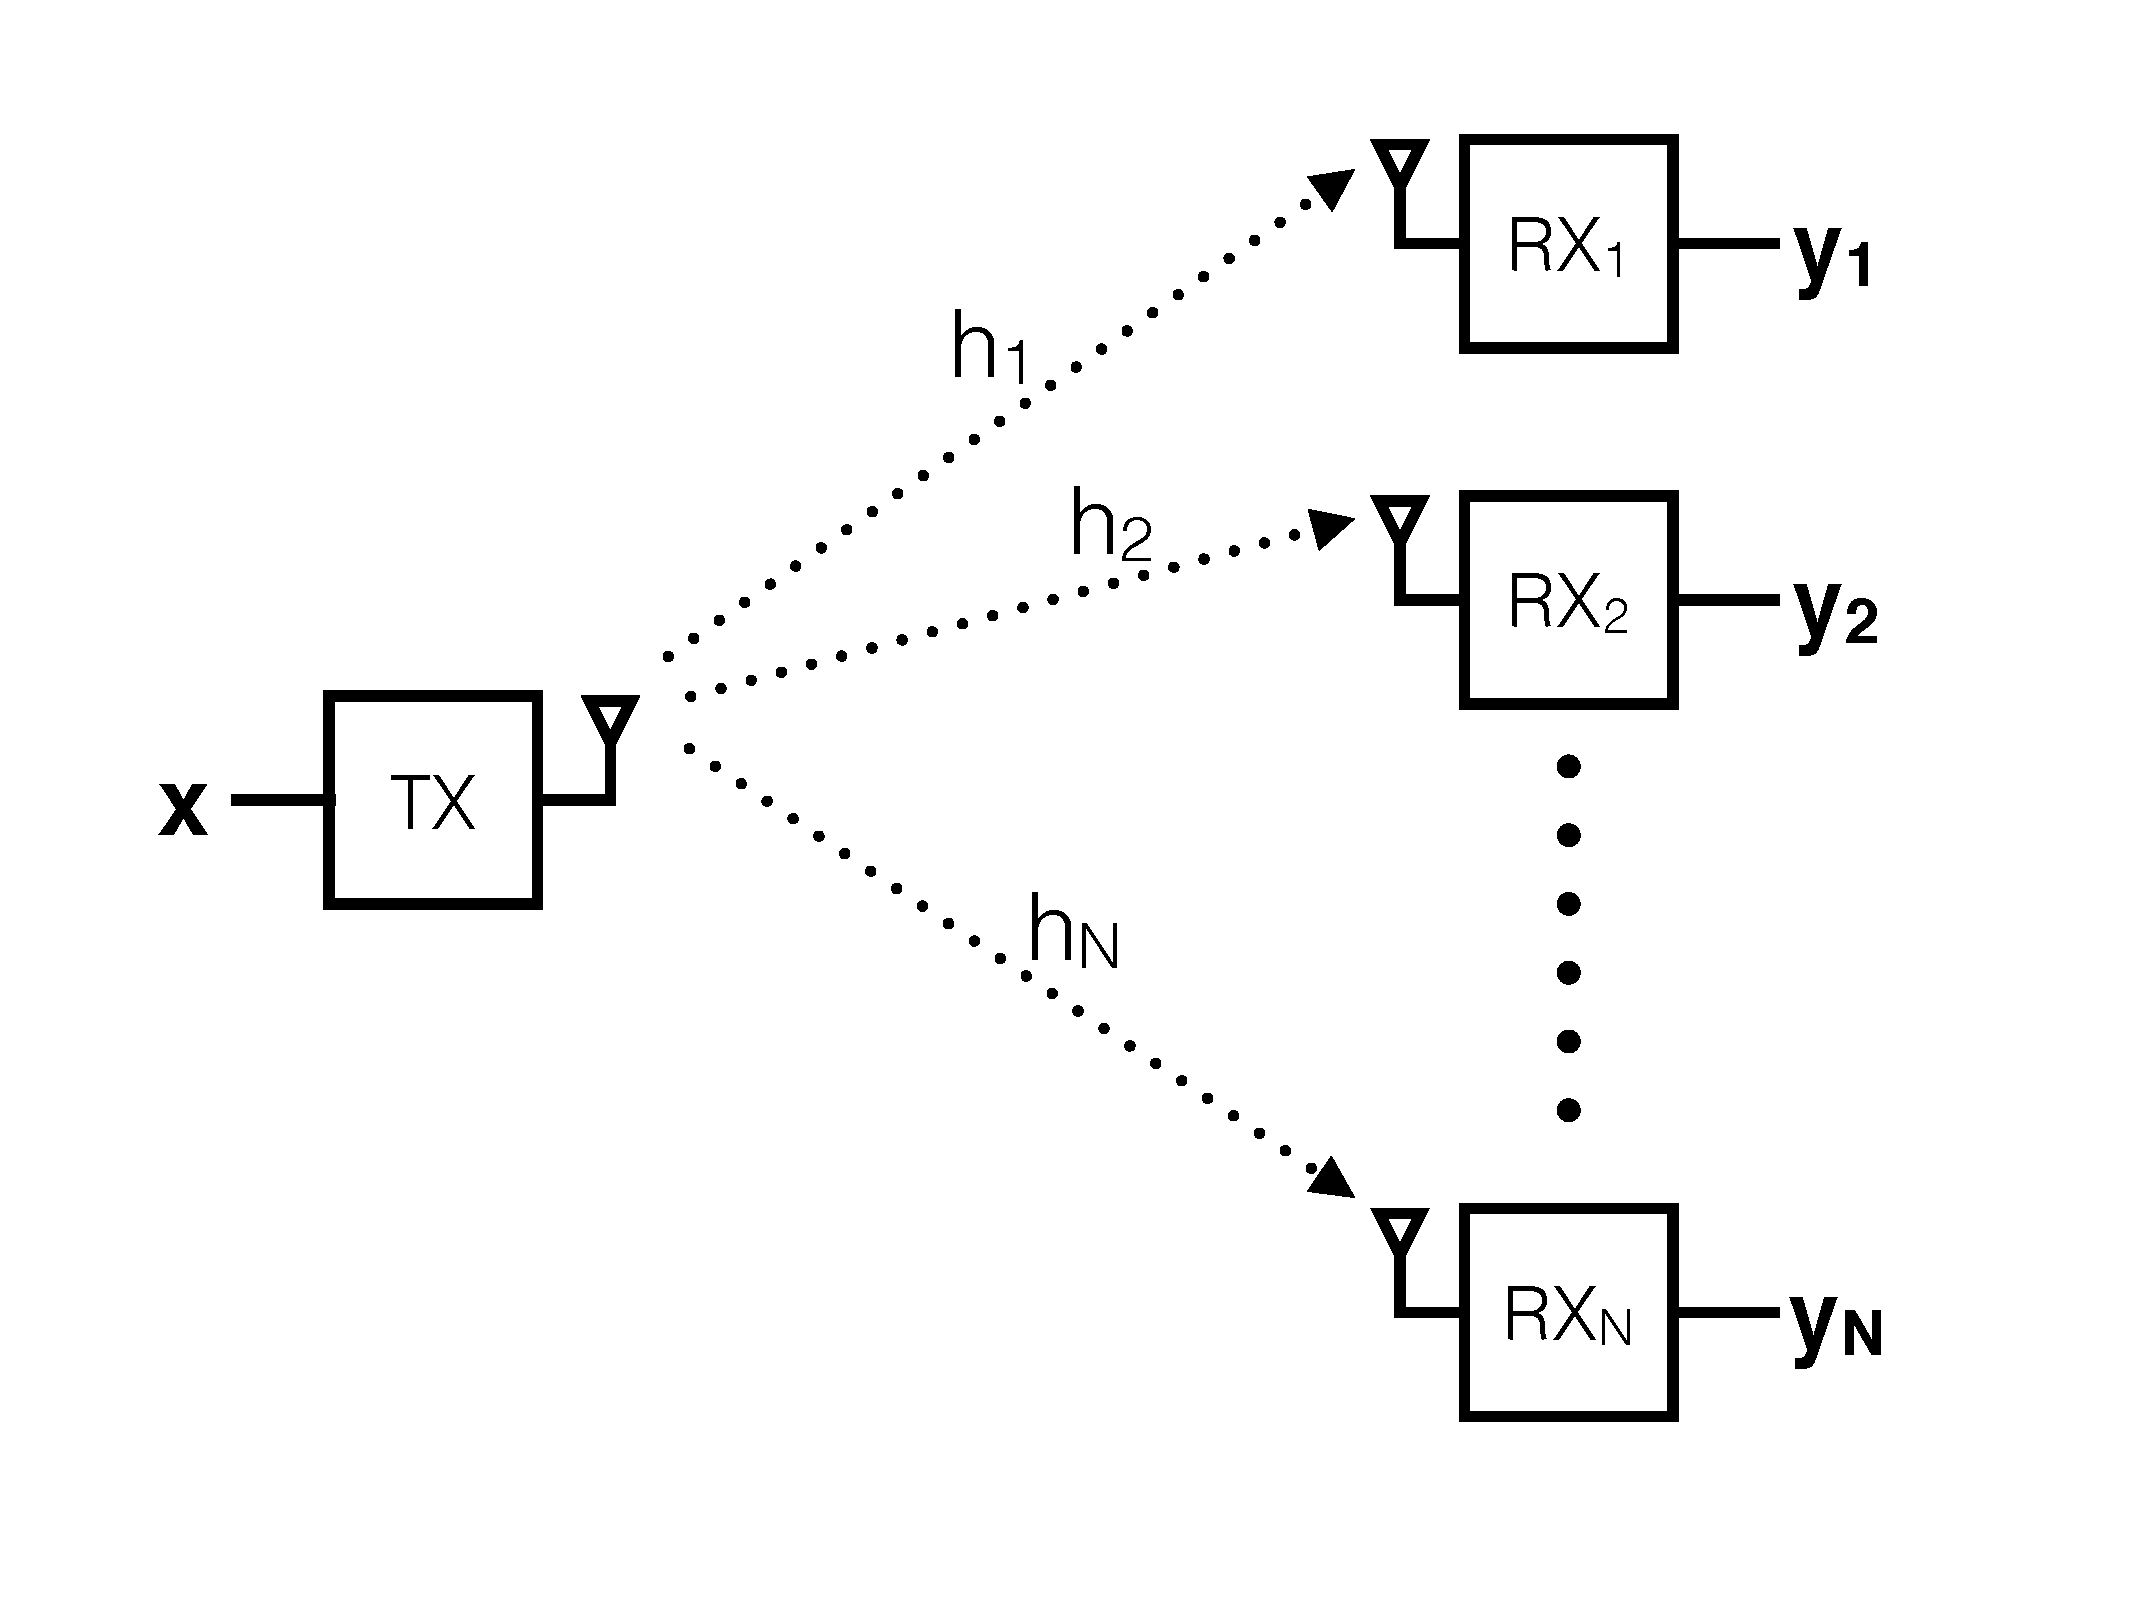
\includegraphics[width=0.45\textwidth]{location-aware-network/figures/SIMO}
    \caption{A single-input multiple-output (SIMO) wireless system}
    \label{fig:simo}
\end{figure}

\subsection{LoRa Modulation}
\label{sec:lora}

\subsection{LoRaWAN}
\label{sec:lorawan}